\documentclass[12pt, a4paper]{article}
\usepackage[utf8]{inputenc}
\usepackage{hyperref}
\usepackage[dvipsnames]{xcolor}
\usepackage{graphicx}
\usepackage{listings}
\usepackage{float}
\usepackage{natbib}
\usepackage{acronym}

\graphicspath{{images/}}

% don't allow to split words over separate lines
\hyphenpenalty 10000
\exhyphenpenalty 10000

\raggedright



\title{Function as a Service}
\author{Xiang Rong Lin}
\date{27.11.2021}

\begin{document}

\maketitle



\newpage
\tableofcontents

\newpage

\section{Einleitung}
bli bla blub

\section{Grundlagen}

\subsection{Cloud computing}
Cloud computing wird vom \ac{NIST} als \cite[ein Modell zur Ermöglichung eines allgegenwärtigen, bequemen und bedarfsgerechten Netzzugang zu einem gemeinsamen Pool konfigurierbarer Rechenressourcen die schnell bereitgestellt und freigegeben werden können mit minimalem Verwaltungsaufwand oder Interaktion mit dem Dienstanbieter]{mell2011nist}.
In dieser Definition gibt es 5 wesentliche Merkmale, 3 Service Modelle und 4 Bereitstellungsmethoden.

\subsection{Merkmale}
Eine kurze Zusammenfassung von \ac{NIST}\cite{mell2011nist}
\subsubsection{On-demand self-service}
Ein Benutzer kann sich selbstständig und automatisiert Ressourcen bereitstellen oder abbestellen ohne eine jegliche Interaktion mit einem Menschen. 

\subsubsection{Broad network access}
Diese Ressourcen sind über ein standardisiertes Interface erreichbar. Dies ist meist das Internet per HTTP.

\subsubsection{Resource pooling}
Der Anbieter dieser Ressourcen verfügt über einen Pool, welche entsprechend der Kundenwünsche zugewiesen werden. Dies passiert in Form von virtuellen Maschinen oder auch Containern.

\subsubsection{Rapid elasticity}
Ressourcen können sehr schnell hinzugefügt und auch wieder entfernt.

\subsubsection{Measured service}
Der Verbrauch von Ressourcen kann sehr genau abgerechnet werden, z.B. in Millisekundenbereich an verwendeter CPU Zeit.

\subsection{Servicemodelle}
In der initialen Definition aus 2011 wurden die 3 Modelle \ac{SaaS}, \ac{PaaS} und \ac{IaaS} beschrieben \cite{mell2011nist}. Inzwischen gibt es eine Vielzahl an Angeboten wie zum Beispiel \ac{BaaS} oder \ac{FaaS}. Es ist auch schon die Rede von \ac{XaaS}, also dass man alles als Service anbieten kann.
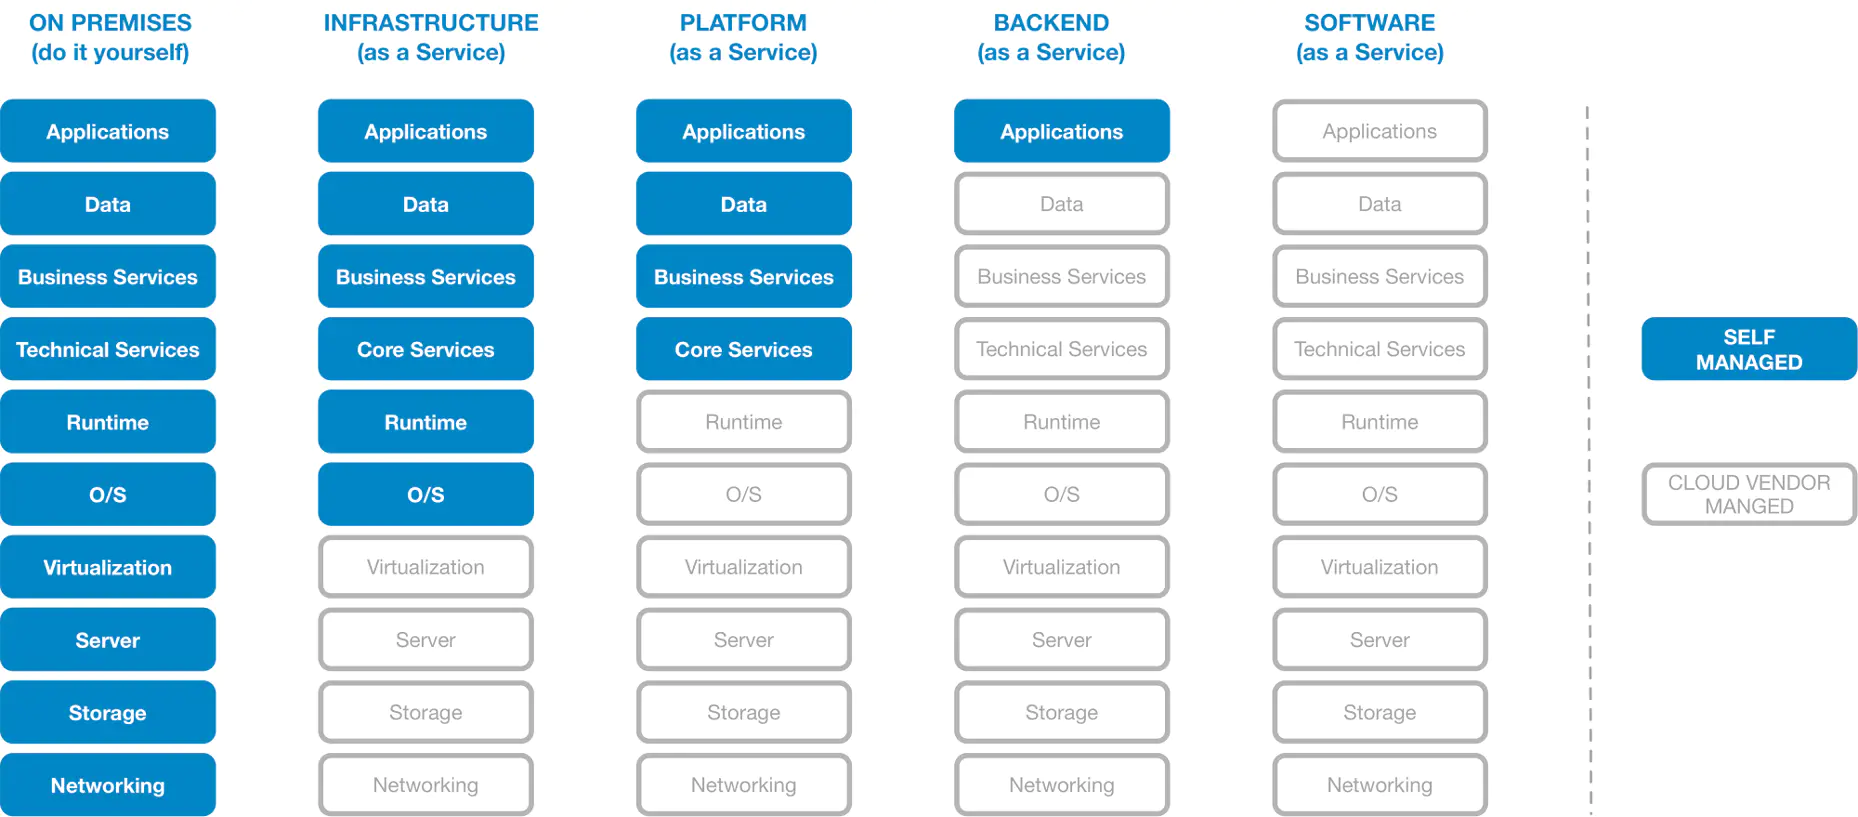
\includegraphics{cloud_service_models.png}\cite{azure2021microsoft}
An obiger Grafik sieht man dass man von \ac{IaaS} über \ac{PaaS} hin zu \ac{SaaS} immer mehr direkt vom Anbieter bereit gestellt kriegt und immer weniger selbst managen muss.
Die neuen Modelle stellen somit nur einen anderen Schnitt der Verantwortlichkeiten dar. So wird bei \ac{DaaS} die Applikation noch feingranularer aufgeteilt in die Datenbank des Providers und der Applikation mit der Businesslogik, welche man selbst implementiert.

\section{Abgrenzung}

\subsection{Serverless}
Serverless bietet außerhalb von Berechnungskapazitäten unter anderem auch Speicher-, Datenbank- und Benachrichtigungsservices an. \footnote{https://www.ibm.com/cloud/learn/faas 27.11.21}
FaaS ist somit nur ein Teil von Serverless, werden fälschlicherweise austauschbar verwendet.


\section{Abkürzungen}
\begin{acronym}
 \acro{NIST}{National Institute of Standards and Technology}
 \acro{SaaS}{Software as a Service}
 \acro{PaaS}{Plattform as a Service}
 \acro{IaaS}{Infrastructure as a Service}
 \acro{BaaS}{Backend as a Service}
 \acro{FaaS}{Function as a Service}
 \acro{DaaS}{Database as a Service}
 \acro{XaaS}{Anything as a Service}
\end{acronym}
\newpage

\bibliography{sources}
\bibliographystyle{abbrv}

\end{document}